\chapter{Metodologia} \label{cap:metodologia}

Este capítulo apresenta a classificação do trabalho e as etapas seguidas em seu desenvolvimento, indicando, em cada etapa, os métodos e as técnicas empregados. O detalhamento da execução de cada etapa se encontra em seu capítulo correspondente.

\section{Caracterização do Trabalho}

O presente trabalho possui uma natureza aplicada, pois se propõe a articular conceitos de Engenharia de modo a solucionar um problema prático, qual seja, o da coleta de telemetria veicular através de um \textit{dongle} OBD-II de maneira segura. Quanto ao objetivo, é exploratório e experimental, sendo qualitativa na modelagem de ameaças e no levantamento de requisitos, e quantitativa na avaliação de desempenho e na análise dos dados coletados.

\section{Etapas do Desenvolvimento}

Foram adotadas as seguintes etapas, que acompanham a ordem dos capítulos, porém não ocorreram de maneira estritamente sequencial. Por exemplo, implementação e testes se deram de maneira incremental, realimentando a especificação e a modelagem de ameaças.

\begin{figure}[htb]
	\centering
	\caption{Etapas do desenvolvimento e realimentações entre elas}
	\label{fig:etapas}
	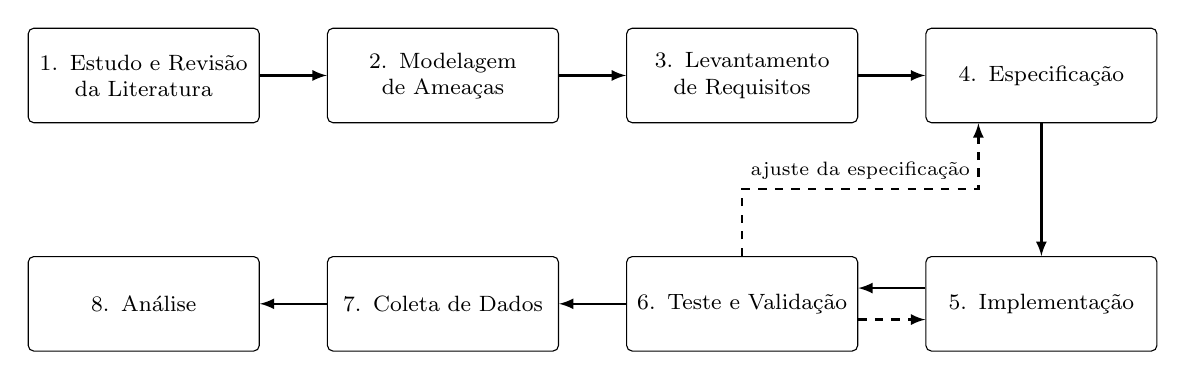
\begin{tikzpicture}[
		etapa/.style={draw, rounded corners=2pt, minimum width=2.9cm, minimum height=1.2cm,
			text width=2.7cm, align=center, font=\footnotesize},
		fluxo/.style={-latex, thick},
		retorno/.style={-latex, thick, dashed}
	]
		% Linha 1: da literatura à especificação
		\node[etapa] (lit) at (0,0) {1. Estudo e Revisão da Literatura};
		\node[etapa] (amea) at (3.8,0) {2. Modelagem de Ameaças};
		\node[etapa] (req) at (7.6,0) {3. Levantamento de Requisitos};
		\node[etapa] (esp) at (11.4,0) {4. Especificação};
 
		% Linha 2 (da direita para a esquerda): da implementação à análise
		\node[etapa] (impl) at (11.4,-2.9) {5. Implementação};
		\node[etapa] (test) at (7.6,-2.9) {6. Teste e Validação};
		\node[etapa] (col) at (3.8,-2.9) {7. Coleta de Dados};
		\node[etapa] (ana) at (0,-2.9) {8. Análise};
 
		% Fluxo principal
		\draw[fluxo] (lit) -- (amea);
		\draw[fluxo] (amea) -- (req);
		\draw[fluxo] (req) -- (esp);
		\draw[fluxo] (esp) -- (impl);
		\draw[fluxo] ([yshift=0.2cm]impl.west) -- ([yshift=0.2cm]test.east);
		\draw[fluxo] (test) -- (col);
		\draw[fluxo] (col) -- (ana);
 
		% Realimentação
		\draw[retorno] ([yshift=-0.2cm]test.east) -- ([yshift=-0.2cm]impl.west);
		\coordinate (c1) at ([yshift=0.85cm]test.north);
		\coordinate (c2) at ([xshift=-0.8cm]esp.south |- c1);
		\draw[retorno] (test.north) -- (c1) -- (c2) -- ([xshift=-0.8cm]esp.south);
		\path (c1) -- (c2) node[midway, above, font=\scriptsize] {ajuste da especificação};
	\end{tikzpicture}
	\legend{Fonte: autores. Setas tracejadas indicam realimentação.}
\end{figure}

\subsection{Estudo e Revisão da Literatura}

Foi realizada uma pesquisa bibliográfica sobre os fundamentos do projeto (CAN, OBD-II, ELM327 e Bluetooth Low Energy), e um esforço de concentrar, em um único lugar, as explicações necessárias para o entendimento do projeto, antevendo possíveis problemas e preocupações que poderiam surgir, e elencando procedimentos padronizados para suas mitigações. O resultado é apresentado no \autoref{cap:conceitos}. 

Além disso, foi realizada uma revisão de trabalhos e artigos que tratam de vulnerabilidades de \textit{dongles} OBD-II, da comunicação segura entre dispositivo e aplicativo, e da coleta e tratamento de dados veiculares, apresentada no \autoref{cap:trabalhosrelacionados}.

\subsection{Modelagem de Ameaças}

A modelagem seguiu quatro passos, a saber: definiu-se a fronteira de confiança; elencaram-se cinco tipos de adversário, de acordo com seu acesso ao sistema; levantaram-se ataques, classificando-os quanto aos componentes atingidos; e, por fim, delimitou-se o escopo de mitigação.

Cada ataque levantado recebe um identificador rastreável no formato AX.Y, e possui seis campos: adversário, pré-condição, método, vulnerabilidade explorada, alvo e efeito. Isto serve de insumo para o desenvolvimento da matriz de rastreabilidade. A descrição completa encontra-se no \autoref{cap:modelagemameacas}.

\subsection{Levantamento de Requisitos}

Os requisitos foram levantados em duas frentes. Os requisitos funcionais foram definidos de modo a capturar o objetivo do sistema: permitir a leitura de códigos de erro (DTCs), a visualização de dados em tempo real, a coleta de leituras de PIDs, o armazenamento e envio de dados ao servidor, e a análise dos dados coletados. Por sua vez, os requisitos não funcionais foram definidos para contemplar a mitigação das ameaças priorizadas na modelagem e para objetivar um desempenho satisfatório, mesmo com as restrições do sistema.

Cada requisito recebe um identificador rastreável, no formato RFXY caso seja funcional, ou RNFXY caso seja não funcional. O levantamento é exposto no \autoref{cap:requisitos}.

\subsection{Especificação}

A especificação partiu da identificação dos componentes do sistema e da interação entre eles. Em seguida, compreendeu-se o fluxo de dados e definiram-se os contratos de dados e a responsabilidade de cada componente do sistema. Cada componente foi então especificado em maior detalhe, de modo a cumprir sua responsabilidade de maneira satisfatória.

No curso deste detalhamento constatou-se que o funcionamento e o desempenho do componente principal, o \textit{dongle}, dependem de um componente externo, o barramento CAN, sobre o qual não se tem controle e cujo comportamento pode variar entre veículos. Para garantir o funcionamento mesmo face às incertezas, fez-se uma modelagem matemática do pior caso da comunicação com o barramento, com base na ISO 15765-4, exposta no \autoref{ap:modelagemcan}. O resultado da especificação é exposto no \autoref{cap:especificacao}.

\subsection{Desenvolvimento}

O \textit{firmware} do \textit{dongle} foi desenvolvido para o ESP32 utilizando o \textit{framework} do Arduino com ambiente de desenvolvimento configurado pelo PlatformIO. A implementação se deu de maneira incremental, e o \textit{app} e o servidor foram desenvolvidos em paralelo.

O simulador de ECU foi incrementado a partir de um projeto de código aberto disponível no GitHub (TODO: COLOCAR LINK DO REPO DO ECUSIM E DAR OS DEVIDOS CRÉDITOS).

A codificação foi feita com auxílio de ferramentas de geração de código com Inteligência Artificial generativa, como o Claude Code, a partir de documentos de especificação previamente escritos com a modelagem definida a partir da especificação. O código gerado foi tratado como proposta e revisado, testado e validado pelos autores. Diagramas que explicam o comportamento do código desenvolvido encontram-se no \autoref{cap:implementacao}.

\subsection{Teste e Validação}

A validação acompanhou a implementação e contou com a estratégia de realismo crescente e com o uso extensivo de \textit{mocks}. O comportamento de coleta e upload do \textit{dongle} pôde ser testados de maneira isolada com a simulação do barramento CAN por meio do software. Já a montagem física dos componentes e a interação com o barramento CAN foram testadas com um emulador de ECU baseado em Arduino, que espelha dados recebidos do BeamNG.drive, um simulador de direção executado em um computador. 

Os testes são funcionais, de desempenho e de segurança, e são definidos e associados aos requisitos que pretendem avaliar, além de receberem um identificador rastreável, utilizado para construir uma matriz de rastreabilidade. 

Para as medições, o \textit{firmware} conta com um modo de depuração que permite a emissão, pela serial, de registros estruturados contendo o momento da ocorrência e o tipo e detalhes do evento (como sincronização, leitura de PID, bloco cheio, \textit{flush} de bloco na flash, upload de bloco, conexão, perda da conexão, entre outros). Isto permite analisar do desempenho e acompanhar a evolução do estado do \textit{dongle}, instante a instante. 

Os testes elencados, o resultado das validações, e as matrizes de rastreabilidade são apresentados no \autoref{cap:validacaotestes}.

\subsection{Coleta de Dados}

A coleta de dados foi realizada na Feira de TCCs da Escola Politécnica da USP, realizada no dia 15/12/2026, utilizando como base um simulador de direção com volante, pedais e câmbio. Os participantes dirigiram no simulador enquanto o \textit{dongle} coletava os parâmetros OBD-II e os dados eram enviados ao servidor por meio do app.  TODO: falar quais dados foram coletados.

% TODO: completar com informações da feira.
\subsection{Análise}

Os dados coletados foram armazenados em um servidor, e são disponibilizados de maneira anonimizada no link (TODO: COLOCAR LINK DE DADOS EXPORTADOS). TODO; FALAR DO SITEZINHO QUE CONSULTA OS DADOS NO SERVIDOR E MOSTRA O COMPORTAMENTO DE DIREÇÃO.